\documentclass{article}
%\documentclass[journal]{IEEEtran}
%\documentclass{report}
%\documentclass{ActaOulu}

\usepackage{graphicx}
\usepackage{listings}
\usepackage{amsmath}

\begin{document}

\title{Report of Project 2}
\author{Wei Jiang}

\maketitle

\begin{abstract}
The Project 2 of PHY607 includes two parts.
In problem \# 1 of Project 2, we evaluate numerical differentiation of arbitrary function and give the relationship between error and step size h.
In problem \# 2 of Project 2, we evaluate numerical integration of arbitrary function, and use Romberg Integration to accelerate the integral process. The result shows that after we use Romberg Integration, the integral needs less steps than before.
\end{abstract}


%\chapter{First Chapter}

\section{Introduction}

In this report of project 1, we have 2 section which are differentiation and integration. There are 3 subsection in each section, the results and discussion are discuss in the following chapter. 


\section{Conclusion}
\subsection{Numerical Differentiation}
\subsection{ Simple numerical derivatives}
In the exercise 1, we calculate the numerical derivative by using one-sided, two-sided and five-point derivatives of a function $f(x)$, which are given by:
\begin{equation}
\begin{split}
f'(x) &\approx \frac{f(x + h) - f(x)}{h} \\
       &\approx \frac{f(x + h) - f(x - h)}{2h}\\
       &\approx \frac{-f(x + 2h) + 8f(x + h) - 8f(x - h) + f(x - 2h)}{12h}\\
\end{split}
\end{equation}
Above equations give the expressions of one-sided, two sided and five point formula for the first derivative of function $f'(x)$. Before give our code and result, let us discuss the formula for the error term as a function of $h$.

As we know, the function $f(x)$ and be expanded as Taylor Series around $x_0$
\begin{equation} \label{eq2}
f(x + h) = f(x) + f'(x)h + \frac{f''(x)}{2}h^2 + \frac{f'''(x)}{3!}h^3 + ...
\end{equation}
\begin{equation} \label{eq3}
f(x - h) = f(x) - f'(x)h + \frac{f''(x)}{2}h^2 - \frac{f'''(x)}{3!}h^3 + ...
\end{equation}
So we can add \ref{eq2} to {eq3} and divided by $2h$, then we have
\begin{equation}
\frac{f(x + h) - f(x - h)}{2h} = f'(x) + \frac{f'''(x)}{3!}h^2 + ...
\end{equation}
Similarly, we can get the expression 
\begin{equation}
\frac{f(x + h) - f(x)}{h} = f'(x) + \frac{f''(x)}{2}h + \frac{f'''(x)}{3!}h^2 + ...
\end{equation}
So we have the expressions for one-sided and two-sided derivatives of function $f(x)$, which are
\begin{equation}
f'(x) = \frac{f(x + h) - f(x)}{h} - \frac{f''(x)}{2}h - ...
\end{equation}
\begin{equation}\label{7}
f'(x) = \frac{f(x + h) - f(x)}{2h} - \frac{f'''(x)}{3!}h^2 - ...
\end{equation}
From above equations we can find that the error of two-sided formula has higher order of $h$ than the one-sided formula, our numerical results also confirm that. The code of our program is listed below


\begin{lstlisting}
#include <stdio.h>
#include <math.h>
#include "stdlib.h"

FILE *fp;

double delta_h1(double (*func)(double x), double x, double h){
    double result1 = (func(x + h) - func(x))/h;
    return result1;
}

double delta_h2(double (*func)(double x), double x, double h){
    double result2 = (func(x + h) - func(x - h))/(2*h);
    return result2;
}

double delta_h5(double (*func)(double x), double x, double h){
    double result5 = (-func(x + 2*h) + 8*func(x + h) 
                         - 8*func(x - h) + func(x - 2*h))/(12*h);
    return result5;
}

double myfun(double x){
    return pow(x, 3);
}

int main(int argc, const char * argv[]) {
    float x[3];
    float h[14] = {5e-15, 3e-15, 2e-15, 1e-15, 1e-10, 
                   1e-5, 0.01, 0.02, 0.03, 0.04, 0.05, 
                    0.07, 0.08, 0.1};

    
    fp = fopen("result_x3.txt", "w");
    for (int i = 0; i < 14; i++) {
        x[0] = fabs(delta_h1(myfun, 2, h[i]) - 12);
        x[1] = fabs(delta_h2(myfun, 2, h[i]) - 12);
        x[2] = fabs(delta_h5(myfun, 2, h[i]) - 12);
        fprintf(fp, "%f %f %f %f\n", h[i], x[0],x[1],x[2]);
        printf("%e %e %e %e\n", h[i], x[0],x[1],x[2]);
    }
    fclose(fp);
    
    return 0;
}
\end{lstlisting} 

This is just the example of our program, because the error depends on the derivative of function $f(x)$, we just set function as $x^3$. From our equation, we know that for one-sided formula, the error should has linear relationship with $h$, for two-sided formula, the error should has parabolic relationship with $h$. We plot the error as $h$ increase, we find that our results are correct and self- consistent.
 
\begin{equation}
Error = -\frac{(b - a)h^2}{12}f'''(\epsilon) =  \mathcal{O}(h^2).
\end{equation}
which shows that the trapezoidal rule is second order accurate. The error was shown in Fig.{\ref{2point}}, which shows that the error increase as $h^2$.
\begin{figure}
    \centering
    \includegraphics[width=4.7in]{x3_1point.eps}
    \caption{Error of one-sided derivative of $x^3$.}
    \label{1point}
\end{figure}
\begin{figure}
    \centering
    \includegraphics[width=4.7in]{x3_2point.eps}
    \caption{Error of two-sided derivative of $x^3$.}
    \label{2point}
\end{figure}

Fig.\ref{1point} and Fig.\ref{2point} give the relationship of error and $h$, it is same as our expect. Also we notice that when $h$ is extreme small, error is large, because the error is so small that it beyond the computer's default accuracy. All the values of errors is listed in the following table
\begin{table}
\begin{center}
\begin{tabular}{ | l | l | l | l | l | | l | | l | l | l | }
\hline
one-sided   & h       &5e-15      & 3e-15      & 1e-15     & 1e-10      &1e-05  &1e-02    &2e-02  \\ 
derivative   & error & 2.76e-01 & 4.34e-01 &  8.32e-7 & 6e-07     & 6e-05  &6.01e-2 &1.2e-01\\ \hline
two-sided   & h       &5e-15       & 3e-15      & 1e-15     & 1e-10     &1e-05   &1e-02    &2e-02  \\ 
derivative   & error & 9.59e-01 & 4.34e-01 &  8.32e-7 & 1.33e-10 & 1e-04 &1e-4      &4e-04\\ \hline                                 
\end{tabular}
\caption {Error of one-sided derivative VS two-sided derivative} \label{tab}
\end{center}
\end{table}

From our discussion, we know that it seems that the more points we choose, the smaller the error is. How about five-point formula? We plot the error as $h$ increase for five point formula using same parameter. We can see that the error really become smaller, and also beyond computer's accuracy.
\begin{table}
\begin{center}
\begin{tabular}{ | l | l | l | l | l | | l | | l | l | l | }
\hline
five point    & h       &5e-15      & 3e-15      & 1e-15     & 1e-10      &1e-05         &2e-02  \\ 
derivative   & error & 2.43e-01 & 6.07e-01 &  3.71e-7 & 8.32e-07 & 5.18e-11  &1.6e-14\\ \hline                                 
\end{tabular}
\caption {Error of five point derivative} \label{tab}
\end{center}
\end{table}


\subsubsection{More accurate formula}
In this exercise, we need to find how much more accurate the extrapolated result becomes with modest values for the step size h. We just need to replace $h$ by $h/2$. Then we have
\begin{equation} \label{9}
f'(x) = \phi(h) - \frac{f''(x)}{3!}\left(\frac{h}{2}\right)^2 - ....
\end{equation}
where $\phi(h)$ = $\frac{f(x + h) - f(x)}{h}$. Then we time Eq.\ref{9} by 4 and subtract Eq.\ref{7}, we have
\begin{equation}
f'(x) = \frac{4 \phi(h/2) - \phi(h)}{3} - K h^4  - ...
\end{equation}
So the error is proportional to $h^4$.

Our code is
\begin{lstlisting}
#include <stdio.h>
#include <math.h>
#include "stdlib.h"

FILE *fp;

double delta_h2(double (*func)(double x), double x, double h){
    double result2 = (func(x + h) - func(x - h))/(2*h);
    return result2;
}

double myfun(double x){
    return exp(x);
}

int main(int argc, const char * argv[]) {
    
    
    fp = fopen("result_x3.txt", "w");
    double x = 2.0, h[6] = {0.05, 0.02, 0.01, 0.005, 0.002, 0.0015};

    for (int i = 0; i < 6; i++) {
        double q = fabs((4*delta_h2(myfun, x, h[i]/2)
                        - delta_h2(myfun, x, h[i]))/3 - exp(x));
        fprintf(fp, "%e %e\n", h[i], q);
        printf("%e %e \n", h[i], q);
    }
    fclose(fp);
    
    return 0;
}
\end{lstlisting}
The result shows that the error is proportional to $h^4$. Our results are listed below:
\begin{table}
\begin{center}
\begin{tabular}{ | l | l | l | l | l | | l | | l | l | l | }
\hline
Richardson    & h       &5e-02      & 2e-02      & 1e-02     & 5e-03      &2e-03         &1.5e-03  \\ 
Extrapolation   & error & 9.62e-08 & 2.46e-09 &  1.54e-10 & 9.68e-14 & 9.8e-13  &4.42e-13\\ \hline                                 
\end{tabular}
\caption {Error of Richardson Extrapolation} \label{tab2}
\end{center}
\end{table}
In Table\ref{tab2}, we fix $h$ use Richardson Extrapolation formula, the error is proportional to $h^4$ which is same as we expected.

\subsubsection{Second derivative}

Finally, we consider the second derivative of a function. We still use eq.\ref{eq2} and eq.\ref{eq3}, then we can find the second derivative of function is
\begin{equation}
f''(x) = \frac{f(x + h) + f(x - h) -2f(x)}{h^2} - \frac{2}{4!}f''''{(\epsilon)}h^2
\end{equation}

where $\epsilon$ is in (x - h, x + h). So the error depends on odd powers of h. If we use $h/2$ replace $h$, we still can get the similar result with the previous
problems. So Richardson Extrapolation can be used here. To find the upper band of the error, we need to calculate $f''''(\epsilon)$, with $\epsilon$ is in (x - h, x + h).
\begin{figure}
    \centering
    \includegraphics[width=4.7in]{xx.eps}
    \caption{Upper band of $sin(x)$.}
    \label{xx}
\end{figure}
 Just take $sin(x)$ function on $\pi/2$ for instance, the 4th derivative of $sin(x)$ is still $sin(x)$ with range from $(\pi/2 - h, \pi/2 + h)$.See Fig.\ref{xx} for more details. We know that for any $\epsilon$ in ($(\pi/2 - h, \pi/2 + h)$, $sin(\pi/2)$ has max value. In this case, the upper band is $h^2/12$. 
 
 To find how the error depends on $h$, we draw Fig.\ref{2deriv}, which shows that the error depends on $h^2$. That is same as our expect. 
 \begin{figure}
    \centering
    \includegraphics[width=4.7in]{2deriv.eps}
    \caption{Error of second derivative of $sin(x)$ at x = 0.5.}
    \label{2deriv}
\end{figure}


\section{Numerical Integration}
\subsubsection{Simple implementation of the trapezoidal rule}

The trapezoidal rule is a technique for approximating the definite integral, $\int_{a}^{b} f(x) dx$. The trapezoidal rule works by approximating the region under the graph of the function $f(x)$ as a trapezoid and calculating its area. It follows that:

\begin{equation}
\int_{a}^{b} f(x) dx \approx  (b - a)[\frac{f(a)+f(b)}{2}].
\end{equation}

For a domain discretized into N equally spaced panels, or N+1 grid points $a  < x_1<...<x_{N} < b$, where the grid spacing is  h = ( b - a )/N, the approximation to the integral becomes,

\begin{equation}\label{eq1}
\begin{split}
\int_{a}^{b} f(x) dx &\approx \frac{h}{2}\sum_{k=1}^{N}(f(x_{k+1}+f(x_k))) \\
& = \frac{b-a}{2N}(f(a) + 2f(x_2) + 2f(x_3) + 2f(x_4) + ... + 2f(x_N-1) +f(b)) \\
& = \frac{h}{2}(f(a) + f(b) + 2 \sum_{i=1}^{N-1}f(x_i))
\end{split}
\end{equation}
where $h = (b - a)/N$.

In exercise 1, we do such a simple implementation of the trapezoidal rule to evaluate $\int_{0}^{1} \exp{-x^2}dx$. Our code is shown as following:


\begin{lstlisting}
#include <stdio.h>
#include <math.h>

FILE *fp;

double trap( double (*func)(double x), double a, double b, double h){
    int i;
    double final = 0, x0, x1 = 0;
    
    x0 = func(a) + func(b);
    for (i = 1; i < (b - a)/h; i++) {
        x1 = x1 + func(a + i*h);
        }
    final = (h/2)*(x0 + 2*x1);
    printf("%e\n", final);
    return final;
}

double myfun(double x){
    return exp(-(x*x));
}


int main(int argc, const char * argv[]) {
    double h = 0.00001;
    double a = 0.0;
    double b = 1.0;
    double ans;
    
    fp = fopen("result.txt", "w");
    
    ans = trap(myfun, a, b, h);
    fprintf(fp, "%f %e\n", h, ans);
    fclose(fp);
}
\end{lstlisting}

Here we set our function as $\exp(-x^2)$, $a = 0$, $b = 1$, $h = 0.00001$, it give the output 7.468241e-01. We know that the analytic expression of the integral is $\frac{1}{2}\sqrt{\pi}Erf(1)$. It seems that our output do make sense.  To test these routines to ensure that they are working. By using a simple function e.g. $f(x) = \sqrt{x}$, determine the rate of convergence (as a function of h). Before give our computational result, it is better to analyze the relationship between error and step size $h$.

The trapezoidal rule approximates the function within each subinterval using the first term in the Taylor series expansion about $x_i$, such that, in the rage $[x_i, x_{i+1}]$,

\begin{equation}
f(x) = f_i + (x - x_i)f'_i + \frac{1}{2}(x - x_i)^2 f"_i + \mathcal{O}((x - x_i)^3).
\end{equation}

Using this approximation, we can evaluate the integral over $[x_i, x_{i+1}]$ with

\begin{equation}
\int_{x_i}^{x_{i+1}} f(x) dx = \int_{x_i}^{x_{i+1}} [f_i + (x - x_i)f'_i + \frac{1}{2}(x - x_i)^2 f"_i]dx.
\end{equation}

Then change variables such that 
\begin{equation}
s = \frac{x - x_i}{x_{i+1} - x_i} = \frac{x - x_i}{h},
\end{equation}

we have 
\begin{equation}
\begin{split}
\int_{x_i}^{x_{i+1}}f(x)dx &= h\int_{0}^{1}(fi + hsf'_i + \frac{1}{2}h^2s^2f''_i)ds\\
                                       &= hsf_i + \frac{1}{2}h^2s^2f'_i + \frac{1}{6}h^3s^3f''_i \vert_{0}^{1} \\
                                       &= hf_i + \frac{1}{2}h^2f'_i + \frac{1}{6}h^3f''_i, 
\end{split}
\end{equation}
Substituting in an approximation for the first derivative
\begin{equation}
f'_i = \frac{f_{i+1} - f_i}{h} - \frac{h}{2}f''_i,
\end{equation}
we have
\begin{equation}
\begin{split}
\int_{x_i}^{x_{i+1}}f(x)dx &= h f_i + \frac{1}{2} h^2 \left( \frac{f_{i +1} - f_i}{h} - \frac{h}{2}f_i \right) + \frac{1}{6}h^3 f_i,\\
                                       &= \frac{1}{2} h (f_i + f_{i+1}) - \frac{1}{12} h^3 f''_i.\\
\end{split}
\end{equation}
The integral over [a, b] is evaluated by taking the sum of the approximate integrals evaluated in each subinterval as
\begin{equation}
\begin{split}
\int_{a}^{b}f(x)dx &= \sum_{i = 0}^{N - 1}\int_{x_i}^{x_{i+1}}f(x)dx,\\
                           &= \sum_{i = 0}^{N - 1}\left[\frac{1}{2}h(f_i + f_{i+1}) - \frac{1}{12}h^3f''_i\right].\\
                           &= \frac{1}{2}h(f_0 + 2f_1 + 2f_2 + ... + 2f_{N-2} + 2f_{N-1} + f_N) - \frac{h^3}{12}\sum_{i=0}^{N-1}f''_i.\\
\end{split}
\end{equation}
So the error term is given is given by
\begin{equation}
\begin{split}
Error &= - \frac{h^3}{12}(f''_0 + f''_1 + f''_2 + .. + f''_{N-1}),\\
         &= - \frac{Nh^3}{12}\left(\frac{f''_0 + f''_1 + f''_2 + .. + f''_{N-1}}{N}\right).\\
\end{split}
\end{equation}
So mean value of $f"_i$ is given by
\begin{equation}
f''(\epsilon) = \left(\frac{f''_0 + f''_1 + f''_2 + .. + f''_{N-1}}{N}\right).
\end{equation}

Therefore, since Nh = (b - a), the error becomes
\begin{equation}
Error = -\frac{(b - a)h^2}{12}f'''(\epsilon) =  \mathcal{O}(h^2).
\end{equation}
which shows that the trapezoidal rule is second order accurate. The error was shown in Fig.1{\ref{fig0}}, which shows that the error increase as $h^2$.
\begin{figure}
    \centering
    \includegraphics[width=4.7in]{error.eps}
    \caption{Error of trapezoidal rule for $\sqrt{x}$  and $e^x$.}
    \label{fig0}
\end{figure}


\subsubsection{Better implementation of the trapezoidal rule}

In exercise 2 we do a better implementation of the trapezoidal rule to evaluate $\int_{0}^{1} \exp{-x^2}dx$. The old version of program in exercise 1 does not have any demand that a certain accuracy be achieved. The new version of program in exercise 2 give a method for guaranteeing a given accuracy with the trapezoidal rule. The integral starts from two points, the trapezoidal rule treats the integration range as a single interval. The integral should then be subdivided into two intervals and the trapezoidal rule used again until the result has converged. Our code is shown as following:

\begin{lstlisting}
#include <stdio.h>
#include <math.h>


double trap( double (*func)(double x), double a, 
                    double b, double vol, int *neval){
    int i, n, step;
    double h, xk, p, ep, y, temp;
    
    n = 1;
    step = *neval;
    i = 0;
    temp = 0;
    h = b - a;
    ep = vol + 1;
    y = h*(func(a) + func(b))/2.0;
    int counter = 2;
    
    while ((ep >= vol)&&counter < step) {
        p = 0.0;
        for (i = 0; i < n; i++) {
            xk = a + (i + 0.5)*h;
            p = p + func(xk);
            counter++;
        }
        y = (y + h*p)/2.0;
        ep = fabs(y-temp);
        temp = y;
        n = n + n;
        h = h/2.0;
        printf("%d %d %e %e\n", counter, n, ep, y);
    }
    return y;
}

double myfun(double x){
    return exp(-(x*x));
}

int main(int argc, const char * argv[]) {
    double vol = 1e-7;
    double a = 0.0;
    double b = 1.0;
    double ans;
    int neval = 10000;
    
    ans = trap(myfun, a, b, vol, &neval);

}

\end{lstlisting}
Here we set accuracy vol equals $10^{-7}$, integrate $e^{-x^2}$ from a = 0 to b = 1. Our result shows that the number of intervals (n) that we divide are 2048, which means we call the function 2049 times. The error which is $g_h(x) - g_{h/2}(x)$, where $g_h(x) = \sum_{i=1}^{N-1}f(x_i)$. From our result, we find error decrease as number of intervals (N) increase. That means the result should  converge as N increase. In next exercise, we use a better approach to evaluate the integration, we will discuss and compare the result in next exercise.

\subsubsection{Romberg Integration}

The Romberg Integration method can be introduced as following, 
as we know
\begin{equation}
\int_{a}^{b} f(x)dx = T_h(x) = \frac{1}{2}h(f(a) + f(b)) + h\sum_{i = 1}^{N - 1}f(x_i) - \frac{b - a}{12}f'''(\epsilon)h^2
\end{equation}
Using steps h and 2h, we have
\begin{equation}
T_h(f) = I(f) + k_2h^2 + k_4h^4 + ... ,
\end{equation}
\begin{equation}
T_2h(f) = I(f) + k_2(2h)^2 + k_4(2h)^4 + ... ,
\end{equation}
Multiplying the first equation by 4 and subtracting from the second one we get
\begin{equation}
4T_h(f) - T_{2h}(f) = 3I(f) + k'_4h^4 + ...
\end{equation}
Thus, we have obtain an integration rule with error proportional to $h^4$ out the one with error proportional to $h^2$. So we can repeat this process, we can get
\begin{equation}
R(n, m) = \frac{1}{4^m - 1}(4^m R(n, m - 1) - R(n - 1, m - 1))
\end{equation}
 Our code is shown as following
 \begin{lstlisting}
 #include <stdio.h>
#include <math.h>


double trap( double (*func)(double x), double a,
                    double b, double tol, int *neval)
{
    int m,n,k;
    double h,ep,p,xk,s,q,y[*neval];
    h = b-a;

    y[0]=h*(func(a)+func(b))/2.0;  // T`1`(h)=1/2(b-a)(f(a)+f(b));
    m = 1;
    n = 1;
    ep = tol+1;
    int counter = 2;
    while((ep >= tol) && (m < *neval))
    {
        p=0.0;
        for(k=0; k<n; k++)
        {
            xk=a + (k + 0.5)*h;     //   n-1
            p = p + func(xk);  // sum over f(xk+h/2),T
            counter++;
        }                      
        p = (y[0] + h*p)/2.0;   //T`m`(h/2),calculate for the area
        s = 1.0;
        for(k=1; k<=m; k++)
        {
            s = 4.0*s;  // pow(4,m)
            q = (s*p-y[k-1])/(s-1.0); 
            y[k-1] = p;
            p=q;
        }
        ep=fabs(q-y[m-1]);  //accuracy
        m=m+1;
        y[m-1]=q;
        n=n+n;   
        h=h/2.0;
    }
    printf("%d, %d, %e, %e\n", n, m, ep, q);
    return q;
}
    
double myfun(double x){
    return exp(-(x*x));
}


int main(int argc, const char * argv[]) {
    double a = 0.0;
    double b = 1.0;
    double tol = 1e-7;
    double ans;
    int neval = 1000;
    
    ans = trap(myfun, a, b, tol, &neval);
    
}
 \end{lstlisting}
Here we set the same parameter as the program in exercise 2, that is a = 0, b = 1, the accuracy equals $10^{-7}$. But we save a lot of step to get the same accuracy. The result shows that we only need call function $exp(-x^2)$ 17 times. We compare these two results in table \ref{tab1}.
\begin{table}
\begin{center}
\begin{tabular}{ | l | l | l | l | l | }
\hline
                         &         h             &   n     & number of recursion &       error \\ \hline
Trapezoidal rule & 9.765620e-04 & 2049  & none & 4.385465e-08 \\ \hline
Romberg          & 1.250000e-01 & 17    &  5 & 4.477063e-10 \\ \hline
\end{tabular}
\caption {Trapezoidal rule VS Romberg} \label{tab1}
\end{center}
\end{table}

In table \ref{tab1}, h is step size, n is number of intervals. As we expect, we can find that error of Trapezoidal Rule approach is proportional to $h^2$, error of Romberg Integration approach is proportional to $h^{10}$. It means our results are correct, and the Romberg Integration really can save a lot of steps for evaluating function for same accuracy, compare with Trapezoidal rule approach.
\end{document}
